% ===========================================================================
%  TikuOS — TikuKits ML: Logistic Regression for Embedded Systems
%  Beamer Presentation
% ===========================================================================
\documentclass[aspectratio=169, 10pt]{beamer}

% ---- Theme ----------------------------------------------------------------
\usetheme{Madrid}
\usecolortheme{whale}
\setbeamertemplate{navigation symbols}{}
\setbeamertemplate{footline}{%
  \leavevmode\hbox{%
    \begin{beamercolorbox}[wd=.33\paperwidth,ht=2.5ex,dp=1ex,center]{author in head/foot}%
      \usebeamerfont{author in head/foot}\insertshortauthor
    \end{beamercolorbox}%
    \begin{beamercolorbox}[wd=.34\paperwidth,ht=2.5ex,dp=1ex,center]{title in head/foot}%
      \usebeamerfont{title in head/foot}\insertshorttitle
    \end{beamercolorbox}%
    \begin{beamercolorbox}[wd=.33\paperwidth,ht=2.5ex,dp=1ex,right]{date in head/foot}%
      \usebeamerfont{date in head/foot}\insertshortdate{}\hspace*{2em}%
      \insertframenumber{}/\inserttotalframenumber\hspace*{2ex}
    \end{beamercolorbox}}%
  \vskip0pt%
}

% ---- Packages -------------------------------------------------------------
\usepackage{listings}
\usepackage{graphicx}
\usepackage{hyperref}
\usepackage{booktabs}
\usepackage{multirow}
\usepackage{tikz}
\usetikzlibrary{arrows.meta, positioning, shapes.geometric, calc,
                decorations.pathreplacing, fit}
\usepackage{amsmath}

% ---- Code listing style ---------------------------------------------------
\lstset{
  basicstyle=\ttfamily\scriptsize,
  keywordstyle=\color{blue}\bfseries,
  commentstyle=\color{gray},
  stringstyle=\color{red!70!black},
  showstringspaces=false,
  breaklines=true,
  frame=single,
  rulecolor=\color{black!30},
  backgroundcolor=\color{blue!3},
  tabsize=4,
}
\lstdefinestyle{cstyle}{
  language=C,
  morekeywords={uint8_t,uint16_t,uint32_t,int32_t,int64_t,
                tiku_kits_ml_elem_t,
                TIKU_KITS_ML_OK,TIKU_KITS_ML_ERR_NULL,
                TIKU_KITS_ML_ERR_SIZE,TIKU_KITS_ML_ERR_PARAM,
                TIKU_KITS_ML_LOGREG_MAX_FEATURES,
                TIKU_KITS_ML_LOGREG_SHIFT,
                NULL},
}

% ---- Metadata -------------------------------------------------------------
\title[TikuKits ML]{TikuKits ML: Logistic Regression for Embedded Systems}
\subtitle{Simple. Ubiquitous. Intelligence, Everywhere.}
\author[Ambuj Varshney]{Ambuj Varshney \\ \texttt{ambuj@tiku-os.org}}
\date{\today}

% ===========================================================================
\begin{document}

% ---------------------------------------------------------------------------
\begin{frame}
\titlepage
\end{frame}

% ---------------------------------------------------------------------------
\begin{frame}{Outline}
\tableofcontents
\end{frame}

% ===========================================================================
\section{Motivation}
% ===========================================================================

\begin{frame}{Why Logistic Regression on MCUs?}
\begin{columns}[T]
\begin{column}{0.48\textwidth}
\begin{block}{Embedded Use Cases}
\begin{itemize}
  \item \textbf{Threshold detection} --- is temperature above safe limit?
  \item \textbf{Fault classification} --- vibration exceeds normal range?
  \item \textbf{Anomaly detection} --- sensor reading suspicious?
  \item \textbf{Probability output} --- confidence-aware decisions
\end{itemize}
\end{block}

\begin{block}{Constraints}
\begin{itemize}
  \item No FPU (16-bit MSP430)
  \item No heap allocation
  \item Limited RAM (2--8\,KB)
  \item Every $\mu$J counts
\end{itemize}
\end{block}
\end{column}

\begin{column}{0.48\textwidth}
\begin{center}
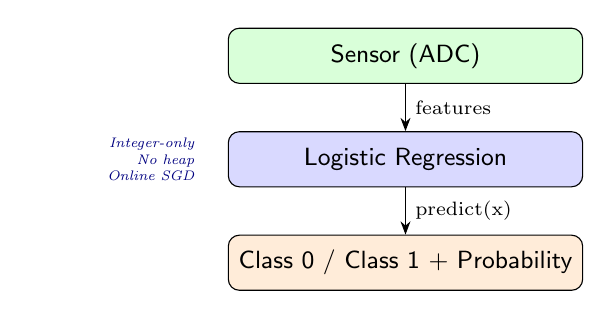
\begin{tikzpicture}[
    >=Stealth, node distance=0.5cm
  ]
  \node[draw, rounded corners, minimum height=0.7cm,
        text centered, font=\small\sffamily, fill=green!15,
        minimum width=4.5cm] (sensor) {Sensor (ADC)};
  \node[draw, rounded corners, minimum height=0.7cm,
        text centered, font=\small\sffamily, fill=blue!15,
        minimum width=4.5cm, below=0.6cm of sensor] (logreg)
    {Logistic Regression};
  \node[draw, rounded corners, minimum height=0.7cm,
        text centered, font=\small\sffamily, fill=orange!15,
        minimum width=4.5cm, below=0.6cm of logreg] (output)
    {Class 0 / Class 1 + Probability};
  \draw[->] (sensor) -- node[right, font=\scriptsize] {features} (logreg);
  \draw[->] (logreg) -- node[right, font=\scriptsize] {predict(x)} (output);

  \node[left=0.3cm of logreg, font=\tiny\itshape, text=blue!50!black,
        text width=2cm, align=right] {Integer-only\\No heap\\Online SGD};
\end{tikzpicture}
\end{center}

\vspace{0.5em}
\begin{alertblock}{Design Goal}
Bring binary logistic regression to devices with \textbf{no floating point},
with online SGD training and probability outputs.
\end{alertblock}
\end{column}
\end{columns}
\end{frame}

% ===========================================================================
\section{Algorithm Theory}
% ===========================================================================

\begin{frame}{Logistic Regression Model}
\begin{columns}[T]
\begin{column}{0.48\textwidth}
\textbf{Decision function:}
\[
  f(\mathbf{x}) = w_0 + \sum_{i=1}^{n} w_i \cdot x_i
\]

\textbf{Probability:}
\[
  P(y=1 \mid \mathbf{x}) = \sigma(f(\mathbf{x}))
\]
where $\sigma(z) = \frac{1}{1+e^{-z}}$.

\vspace{0.5em}
\textbf{Classification:}
\[
  \hat{y} = \begin{cases} 1 & \text{if } \sigma(f(\mathbf{x})) \geq 0.5 \\ 0 & \text{otherwise} \end{cases}
\]

\textbf{SGD update} for sample $(\mathbf{x}, y)$:
\[
  w_j \leftarrow w_j + \eta \cdot (y - \hat{p}) \cdot x_j
\]
\end{column}

\begin{column}{0.48\textwidth}
\begin{center}
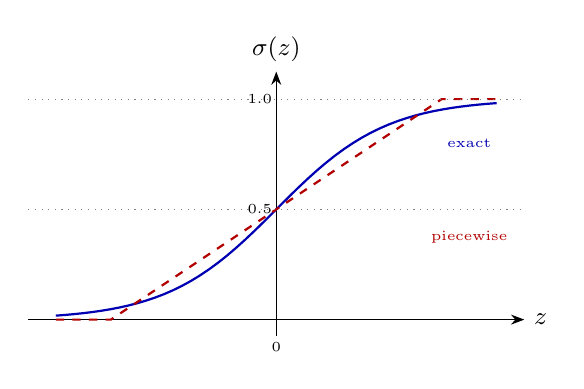
\begin{tikzpicture}[>=Stealth, scale=0.7]
  % Axes
  \draw[->] (-4.5,0) -- (4.5,0) node[right] {\small $z$};
  \draw[->] (0,-0.3) -- (0,4.5) node[above] {\small $\sigma(z)$};

  % Sigmoid curve (approximate)
  \draw[thick, blue!70!black, domain=-4:4, samples=50]
    plot (\x, {4/(1+exp(-\x))});

  % Piecewise linear approximation
  \draw[thick, red!70!black, dashed]
    (-4, 0) -- (-3, 0) -- (3, 4) -- (4, 4);

  % Labels
  \node[font=\tiny] at (0, -0.5) {0};
  \node[font=\tiny] at (-0.3, 2) {0.5};
  \draw[dotted, gray] (-4.5, 2) -- (4.5, 2);
  \draw[dotted, gray] (-4.5, 4) -- (4.5, 4);
  \node[font=\tiny] at (-0.3, 4) {1.0};

  % Legend
  \node[font=\tiny, blue!70!black] at (3.5, 3.2) {exact};
  \node[font=\tiny, red!70!black] at (3.5, 1.5) {piecewise};
\end{tikzpicture}
\end{center}

\vspace{0.3em}
\begin{block}{Integer Sigmoid Approximation}
3-piece piecewise linear in Q(shift):
\begin{itemize}
  \item $z \leq -4$: return $0$
  \item $-4 < z < 4$: return $z/8 + 0.5$
  \item $z \geq 4$: return $1$
\end{itemize}
No \texttt{exp()}, no FPU needed.
\end{block}
\end{column}
\end{columns}
\end{frame}

% ===========================================================================
\section{Data Structure}
% ===========================================================================

\begin{frame}[fragile]{The \texttt{tiku\_kits\_ml\_logreg} Structure}
\begin{columns}[T]
\begin{column}{0.48\textwidth}
\begin{lstlisting}[style=cstyle,
  title={ml/classification/tiku\_kits\_ml\_logreg.h}]
struct tiku_kits_ml_logreg {
    /* bias + feature weights Q(shift) */
    int32_t weights[
        TIKU_KITS_ML_LOGREG_MAX_FEATURES
        + 1];
    uint8_t  n_features;
    uint8_t  shift;
    int32_t  learning_rate;
    uint16_t n;
};
\end{lstlisting}

\vspace{0.3em}
\textbf{Memory footprint:}\\
$(8+1) \times 4 + 1 + 1 + 4 + 2 = 44$ bytes per model.\\
All statically allocated --- no heap.
\end{column}

\begin{column}{0.48\textwidth}
\textbf{Weight vector layout:}
\begin{center}
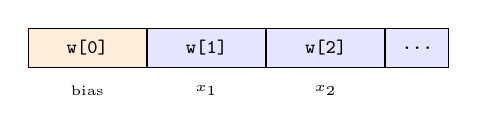
\begin{tikzpicture}[
    >=Stealth, node distance=0.15cm
  ]
  \node[draw, minimum width=1.5cm, minimum height=0.5cm,
        fill=orange!15, font=\scriptsize\ttfamily] (w0) {w[0]};
  \node[draw, minimum width=1.5cm, minimum height=0.5cm,
        fill=blue!10, font=\scriptsize\ttfamily, right=0cm of w0] (w1) {w[1]};
  \node[draw, minimum width=1.5cm, minimum height=0.5cm,
        fill=blue!10, font=\scriptsize\ttfamily, right=0cm of w1] (w2) {w[2]};
  \node[draw, minimum width=0.8cm, minimum height=0.5cm,
        fill=blue!10, font=\scriptsize\ttfamily, right=0cm of w2] (wd) {...};

  \node[font=\tiny, below=0.1cm of w0] {bias};
  \node[font=\tiny, below=0.1cm of w1] {$x_1$};
  \node[font=\tiny, below=0.1cm of w2] {$x_2$};
\end{tikzpicture}
\end{center}

\vspace{1em}
\begin{block}{Online Learning}
\begin{itemize}
  \item Train one sample at a time
  \item No sample buffer needed
  \item Default learning rate: $\sim 0.1$ in Q8
  \item Labels: $y \in \{0, 1\}$
\end{itemize}
\end{block}
\end{column}
\end{columns}
\end{frame}

% ===========================================================================
\section{API Reference}
% ===========================================================================

\begin{frame}[fragile]{Complete API}
\begin{table}
\centering
\small
\begin{tabular}{@{}lp{8cm}@{}}
\toprule
\textbf{Function} & \textbf{Description} \\
\midrule
\texttt{tiku\_kits\_ml\_logreg\_init(lr, nf, sh)}
  & Initialize model with \texttt{nf} features, Q-format \texttt{sh} \\
\texttt{tiku\_kits\_ml\_logreg\_reset(lr)}
  & Zero all weights, reset training count \\
\texttt{tiku\_kits\_ml\_logreg\_set\_lr(lr, rate)}
  & Set learning rate in Q(shift) \\
\midrule
\texttt{tiku\_kits\_ml\_logreg\_train(lr, x, y)}
  & One SGD step; label $y \in \{0,1\}$ \\
\texttt{tiku\_kits\_ml\_logreg\_predict(lr, x, \&result)}
  & Binary prediction: 0 or 1 \\
\texttt{tiku\_kits\_ml\_logreg\_predict\_proba(lr, x, \&prob)}
  & Probability in Q(shift); range $[0, 2^{\text{shift}}]$ \\
\midrule
\texttt{tiku\_kits\_ml\_logreg\_get\_weights(lr, w)}
  & Export weight vector (bias + features) \\
\texttt{tiku\_kits\_ml\_logreg\_set\_weights(lr, w)}
  & Load pre-trained weights \\
\texttt{tiku\_kits\_ml\_logreg\_count(lr)}
  & Number of training samples seen \\
\bottomrule
\end{tabular}
\end{table}

\vspace{0.3em}
\begin{alertblock}{Probability Output}
\texttt{predict\_proba()} returns the sigmoid approximation of $f(\mathbf{x})$
in Q(shift). With shift=8, a return value of 128 means 50\% confidence.
\end{alertblock}
\end{frame}

% ===========================================================================
\section{Configuration}
% ===========================================================================

\begin{frame}[fragile]{Compile-Time Configuration}
\begin{columns}[T]
\begin{column}{0.48\textwidth}
\begin{lstlisting}[style=cstyle,
  title={Configurable parameters}]
/* Maximum input features */
#ifndef TIKU_KITS_ML_LOGREG_MAX_FEATURES
#define TIKU_KITS_ML_LOGREG_MAX_FEATURES 8
#endif

/* Default Q-format shift */
#ifndef TIKU_KITS_ML_LOGREG_SHIFT
#define TIKU_KITS_ML_LOGREG_SHIFT 8
#endif
\end{lstlisting}

\vspace{0.3em}
\textbf{Defaults at init:}
\begin{itemize}
  \item Learning rate: $(1 \ll \text{shift}) / 10 \approx 0.1$
  \item All weights zeroed
\end{itemize}
\end{column}

\begin{column}{0.48\textwidth}
\begin{lstlisting}[style=cstyle,
  title={Runtime configuration}]
struct tiku_kits_ml_logreg lr;

/* 3 features, 8-bit Q-format */
tiku_kits_ml_logreg_init(&lr, 3, 8);

/* Tune learning rate: ~0.05 */
tiku_kits_ml_logreg_set_lr(&lr, 13);

/* Or load pre-trained weights */
int32_t w[] = {128, 256, -128, 64};
tiku_kits_ml_logreg_set_weights(
    &lr, w);
\end{lstlisting}

\vspace{0.3em}
\begin{table}
\centering
\scriptsize
\begin{tabular}{@{}rrr@{}}
\toprule
\textbf{Shift} & \textbf{Scale} & \textbf{Resolution} \\
\midrule
4  & 16     & 0.0625 \\
8  & 256    & 0.0039 \\
12 & 4096   & 0.00024 \\
\bottomrule
\end{tabular}
\end{table}
\end{column}
\end{columns}
\end{frame}

% ===========================================================================
\section{Implementation Details}
% ===========================================================================

\begin{frame}[fragile]{Integer Sigmoid and Dot Product}
\begin{columns}[T]
\begin{column}{0.48\textwidth}
\begin{lstlisting}[style=cstyle,
  title={Dot product --- int64 accumulation}]
static int32_t dot_product(
    const struct tiku_kits_ml_logreg *lr,
    const tiku_kits_ml_elem_t *x)
{
    int64_t acc;
    uint8_t i;

    acc = (int64_t)lr->weights[0]; /*bias*/
    for (i = 0; i < lr->n_features; i++) {
        acc += (int64_t)lr->weights[i + 1]
               * (int64_t)x[i];
    }
    return (int32_t)(acc >> lr->shift);
}
\end{lstlisting}
\end{column}

\begin{column}{0.48\textwidth}
\begin{lstlisting}[style=cstyle,
  title={Piecewise sigmoid approximation}]
static int32_t sigmoid_q(
    int32_t z, uint8_t shift)
{
    int32_t one_q = (int32_t)(1 << shift);
    int32_t four_q = 4 * one_q;
    int32_t half_q = one_q / 2;

    if (z <= -four_q)
        return 0;
    if (z >= four_q)
        return one_q;

    /* Linear: z/8 + 0.5 */
    return half_q
           + (z * one_q) / (8 * one_q);
}
\end{lstlisting}
\end{column}
\end{columns}

\vspace{0.3em}
\begin{block}{Why Piecewise Linear?}
The exact sigmoid requires \texttt{exp()} which is unavailable on MSP430.
A 3-piece linear approximation captures the S-shape with only integer
multiply and divide --- sufficient for binary classification on embedded targets.
\end{block}
\end{frame}

% ---------------------------------------------------------------------------
\begin{frame}[fragile]{SGD Training Step}
\begin{lstlisting}[style=cstyle,
  title={tiku\_kits\_ml\_logreg.c --- train}]
int tiku_kits_ml_logreg_train(struct tiku_kits_ml_logreg *lr,
                              const tiku_kits_ml_elem_t *x, uint8_t y)
{
    int32_t z, p_q, error;
    int64_t lr_err;
    uint8_t i;

    /* Forward: dot product then sigmoid */
    z   = dot_product(lr, x);
    p_q = sigmoid_q(z, lr->shift);

    /* Error: target - predicted (in Q(shift)) */
    error = ((int32_t)(y ? (1 << lr->shift) : 0)) - p_q;

    /* Gradient descent update */
    lr_err = ((int64_t)lr->learning_rate * (int64_t)error) >> lr->shift;

    lr->weights[0] += (int32_t)lr_err;                    /* bias */
    for (i = 0; i < lr->n_features; i++) {
        lr->weights[i + 1] += (int32_t)(lr_err * (int64_t)x[i]);
    }

    lr->n++;
    return TIKU_KITS_ML_OK;
}
\end{lstlisting}
\end{frame}

% ===========================================================================
\section{Examples}
% ===========================================================================

\begin{frame}[fragile]{Example 1: Temperature Alarm}
\begin{lstlisting}[style=cstyle,
  title={examples/example\_ml\_logreg.c --- classify hot vs. safe}]
struct tiku_kits_ml_logreg lr;
uint8_t result;

tiku_kits_ml_logreg_init(&lr, 1, 8);   /* 1 feature, Q8 */

/* Train: temperature (deci-C) -> safe(0) / hot(1) */
static const int32_t temps[]  = {200, 220, 240, 300, 320, 340};
static const uint8_t labels[] = {  0,   0,   0,   1,   1,   1};

uint8_t epoch, s;
for (epoch = 0; epoch < 30; epoch++) {
    for (s = 0; s < 6; s++) {
        tiku_kits_ml_logreg_train(&lr, &temps[s], labels[s]);
    }
}

/* Predict on new reading */
int32_t new_temp = 280;
tiku_kits_ml_logreg_predict(&lr, &new_temp, &result);
/* result: 0 or 1 depending on learned boundary */
\end{lstlisting}
\end{frame}

% ---------------------------------------------------------------------------
\begin{frame}[fragile]{Example 2: Pre-Trained Vibration Classifier}
\begin{columns}[T]
\begin{column}{0.52\textwidth}
\begin{lstlisting}[style=cstyle,
  title={Deploy with pre-computed weights}]
struct tiku_kits_ml_logreg lr;
uint8_t result;
int32_t prob;

tiku_kits_ml_logreg_init(&lr, 2, 8);

/* Load pre-trained weights:
 * bias = -5.0, w1 = +3.0, w2 = +2.0
 * in Q8: -1280, +768, +512 */
int32_t w[] = {-1280, 768, 512};
tiku_kits_ml_logreg_set_weights(&lr, w);

/* Classify vibration sample */
tiku_kits_ml_elem_t x[] = {3, 2};
tiku_kits_ml_logreg_predict(&lr, x,
                            &result);
tiku_kits_ml_logreg_predict_proba(&lr, x,
                                  &prob);

/* prob gives confidence in Q8
 * 256 = 100%, 128 = 50% */
\end{lstlisting}
\end{column}

\begin{column}{0.44\textwidth}
\begin{center}
\begin{tikzpicture}[>=Stealth, scale=0.65]
  % Axes
  \draw[->] (0,0) -- (5.5,0) node[right] {\tiny $x_1$};
  \draw[->] (0,0) -- (0,5) node[above] {\tiny $x_2$};

  % Decision boundary: -5 + 3*x1 + 2*x2 = 0
  % => x2 = (5 - 3*x1) / 2
  \draw[thick, blue!70!black] (0, 2.5) -- (1.67, 0);

  % Class 0 points
  \fill[green!60!black] (0.2, 0.5) circle (3pt);
  \fill[green!60!black] (0.5, 0.3) circle (3pt);
  \fill[green!60!black] (0.3, 1.0) circle (3pt);

  % Class 1 points
  \fill[red!70!black] (2.5, 2.0) circle (3pt);
  \fill[red!70!black] (3.0, 3.0) circle (3pt);
  \fill[red!70!black] (4.0, 2.5) circle (3pt);

  % Labels
  \node[font=\tiny, green!50!black] at (0.8, 1.5) {safe};
  \node[font=\tiny, red!60!black] at (3.5, 3.5) {fault};
  \node[font=\tiny, blue!60!black, rotate=-55] at (1.2, 1.8) {boundary};
\end{tikzpicture}
\end{center}

\vspace{0.5em}
\begin{block}{Pre-Trained Deployment}
Train offline (PC/cloud), export weights,
deploy on MCU with \texttt{set\_weights()}.
Zero training cost on-device.
\end{block}
\end{column}
\end{columns}
\end{frame}

% ===========================================================================
\section{Test Suite}
% ===========================================================================

\begin{frame}{Test Cases Overview}
\begin{table}
\centering
\small
\begin{tabular}{@{}clp{7cm}@{}}
\toprule
\textbf{\#} & \textbf{Test Function} & \textbf{What It Verifies} \\
\midrule
1 & \texttt{test\_kits\_ml\_logreg\_init}
  & Proper initialization, parameter validation \\
2 & \texttt{test\_kits\_ml\_logreg\_pretrained}
  & Pre-loaded weights produce correct predictions \\
3 & \texttt{test\_kits\_ml\_logreg\_sigmoid\_saturation}
  & Extreme inputs saturate to 0 or 1 \\
4 & \texttt{test\_kits\_ml\_logreg\_sigmoid\_midpoint}
  & Zero input gives $\sim$0.5 probability \\
5 & \texttt{test\_kits\_ml\_logreg\_training}
  & SGD convergence on linearly separable data \\
6 & \texttt{test\_kits\_ml\_logreg\_two\_features}
  & Multi-feature classification \\
7 & \texttt{test\_kits\_ml\_logreg\_reset}
  & Reset clears weights and count \\
8 & \texttt{test\_kits\_ml\_logreg\_learning\_rate}
  & Custom learning rate accepted \\
9 & \texttt{test\_kits\_ml\_logreg\_null\_inputs}
  & All functions reject NULL with ERR\_NULL \\
\bottomrule
\end{tabular}
\end{table}
\end{frame}

% ===========================================================================
\section{Summary}
% ===========================================================================

\begin{frame}{Summary}
\begin{columns}[T]
\begin{column}{0.48\textwidth}
\begin{block}{What We Built}
\begin{itemize}
  \item Binary logistic regression classifier
  \item Integer-only piecewise sigmoid
  \item Online SGD training (one sample at a time)
  \item 44 bytes of state, no heap
  \item Probability output in Q(shift)
\end{itemize}
\end{block}

\begin{block}{Key Design Choices}
\begin{itemize}
  \item 3-piece linear sigmoid avoids \texttt{exp()}
  \item \texttt{int64\_t} dot product prevents overflow
  \item Separate \texttt{predict()} and \texttt{predict\_proba()}
  \item Pre-trained weight loading supported
\end{itemize}
\end{block}
\end{column}

\begin{column}{0.48\textwidth}
\begin{block}{Use Cases}
\begin{itemize}
  \item Temperature threshold alarms
  \item Vibration fault detection
  \item Motion/gesture binary classification
  \item Confidence-aware embedded decisions
\end{itemize}
\end{block}

\begin{block}{Files}
\scriptsize
\begin{tabular}{@{}lp{4.5cm}@{}}
Header: & \texttt{ml/classification/tiku\_kits\_ml\_logreg.h} \\
Source: & \texttt{ml/classification/tiku\_kits\_ml\_logreg.c} \\
Tests: & \texttt{tests/ml/test\_kits\_ml\_logreg.c} \\
Example: & \texttt{examples/example\_ml\_logreg.c} \\
\end{tabular}
\end{block}
\end{column}
\end{columns}
\end{frame}

% ---------------------------------------------------------------------------
\begin{frame}{Thank You}
\begin{center}
\Large\textbf{TikuKits ML: Logistic Regression}\\[0.5em]
\normalsize Integer-Only Machine Learning for Physical AI Endpoints\\[1.5em]

\begin{tabular}{rl}
  Repository: & \url{https://github.com/tikuos/tikuOS} \\
  License:    & Apache 2.0 \\
  Common:     & \texttt{tikukits/ml/tiku\_kits\_ml.h} \\
  Header:     & \texttt{tikukits/ml/classification/tiku\_kits\_ml\_logreg.h} \\
  Source:     & \texttt{tikukits/ml/classification/tiku\_kits\_ml\_logreg.c} \\
  Tests:      & \texttt{tikukits/tests/ml/test\_kits\_ml\_logreg.c} \\
  Examples:   & \texttt{tikukits/examples/example\_ml\_logreg.c} \\
\end{tabular}
\end{center}
\end{frame}

\end{document}
